\documentclass[border=10pt,12pt]{standalone}
\usepackage{times}
\usepackage{amsmath,amssymb}
\usepackage{graphicx}
\usepackage{tikz}
\usetikzlibrary{arrows.meta, positioning, shadows}
% Drop a logo file here to replace the generic chip: assets/fig/llm-logo.png or .pdf
\newcommand{\logopath}{llm-logo.png}
\hyphenpenalty=10000 \exhyphenpenalty=10000
\begin{document}
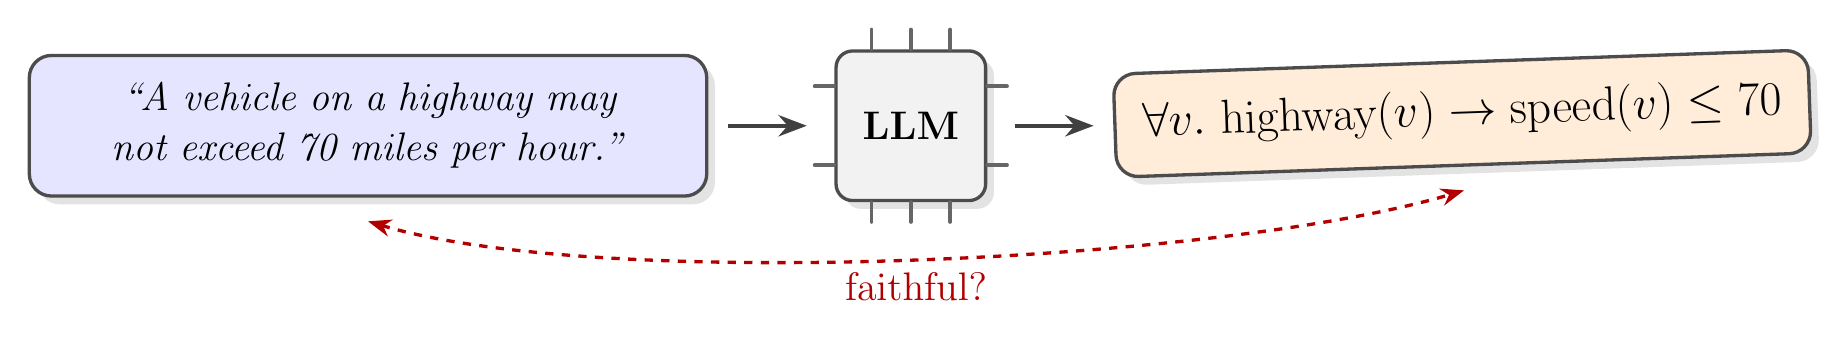
\begin{tikzpicture}[>=Stealth, font=\Large,
  card/.style={draw=black!70, line width=1.2pt, rounded corners=8pt, inner sep=10pt,
               drop shadow={opacity=0.22, shadow xshift=3pt, shadow yshift=-3pt}},
  nlcard/.style={card, fill=blue!10, text width=7.9cm, align=center, font=\Large\itshape},
  fmcard/.style={card, fill=orange!15, align=center, font=\LARGE, rotate=2},
  chip/.style={draw=black!70, line width=1.2pt, rounded corners=6pt, fill=black!5,
               minimum size=1.9cm, font=\Large\bfseries, inner sep=4pt,
               drop shadow={opacity=0.22, shadow xshift=3pt, shadow yshift=-3pt}},
  pin/.style={draw=black!60, line width=1.4pt, line cap=round},
  arr/.style={->, line width=1.6pt, black!75},
]
\node[nlcard] (nl) {``A vehicle on a highway may not exceed 70 miles per hour.''};
\node[chip, right=1.6cm of nl] (llm)
  {\IfFileExists{\logopath}{\includegraphics[width=1.4cm]{\logopath}}{LLM}};
\foreach \y in {-0.5,0.5} {
  \draw[pin] ([yshift=\y cm]llm.west) -- ++(-0.25,0);
  \draw[pin] ([yshift=\y cm]llm.east) -- ++(0.25,0);
}
\foreach \x in {-0.5,0,0.5} {
  \draw[pin] ([xshift=\x cm]llm.north) -- ++(0,0.25);
  \draw[pin] ([xshift=\x cm]llm.south) -- ++(0,-0.25);
}
\node[fmcard, right=1.6cm of llm] (fm)
  {$\forall v.\ \mathrm{highway}(v) \rightarrow \mathrm{speed}(v) \le 70$};
\draw[arr] ([xshift=0.25cm]nl.east) -- ([xshift=-0.35cm]llm.west);
\draw[arr] ([xshift=0.35cm]llm.east) -- ([xshift=-0.25cm]fm.west);
\draw[{Stealth}-{Stealth}, dashed, line width=1.2pt, red!70!black]
  ([yshift=-0.3cm]nl.south) .. controls +(3.0,-0.9) and +(-3.0,-0.9) ..
  node[below=1pt, text=red!70!black] {faithful?} ([yshift=-0.3cm]fm.south);
\end{tikzpicture}
\end{document}
